\documentclass{article}
\usepackage[utf8]{inputenc}
\usepackage{graphicx}
\usepackage{hyperref}
\usepackage{fancyhdr}
\usepackage[font=small,skip=0pt]{caption}
\pagestyle{fancy}

\fancyhead[LE,RO]{Jesse Both}
\fancyhead[LO,RE]{ASSIGNMENT}


\hypersetup{
    colorlinks,
    citecolor=black,
    filecolor=black,
    linkcolor=black,
    urlcolor=black
}
\graphicspath{ {/graphics/} }
\title{\Huge{\textbf{COURSE}  \\* ASSIGNMENT \\~\\ \textbf{SUB \\* TITLE}}}

\date{} %remove date from make title


%image
% \begin{figure}[h!]
%   \begin{center}
%     \includegraphics[height=5cm]{graphics/().png}
%   \end{center}
%   \caption{CAPTION}
%   \label{fig:LABEL}
% \end{figure}

% Title Page
\begin{document}
%     \maketitle
%     \vfill 
%     {\Large\centering\textbf{Jesse Both  \\~\\}\par}

%     {\Large\centering{Fall 2021}\par}
%     {\large\centering{\today}\par}

%     \newpage
%     \begin{center}
%         \tableofcontents
%     \end{center}
% \newpage
\setcounter{secnumdepth}{-1}

\section{Step 1}
    \subsection{Microgrid Block Diagram}
    \begin{figure}[h!]
    \begin{center}
        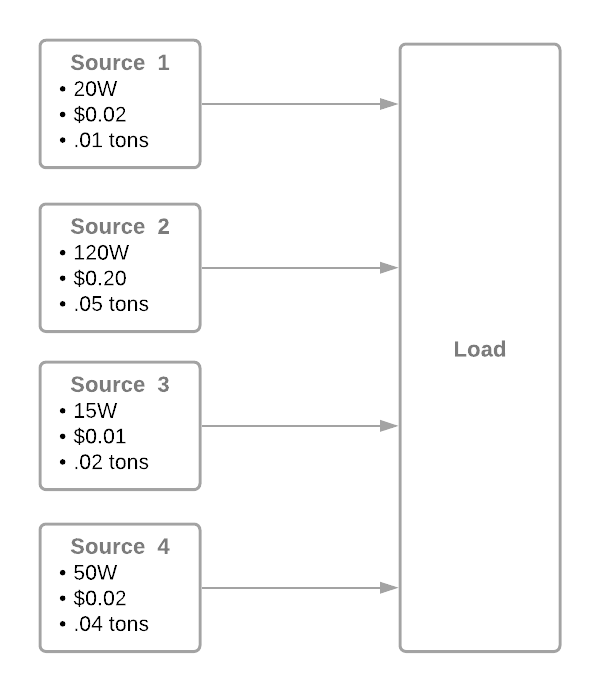
\includegraphics[height=8cm]{graphics/block_diagram.png}
    \end{center}
    \caption{Block Diagram}
    \label{fig:block}
    \end{figure}

    \subsection{Load Time Series}
    This time series was designed by deciding with the idea that the power is being sent to a residential area.  The usage would be low in the middle
    of the night and high when residents are home from work.  It would gradually
    increase/decrease throughout the other parts of the day.  The assumption
    is that a week days are being explored.

    To find the values, a range was given for each hour through out the day.
    A value for each hour within these ranges is randomly selected.  A set
    number of days can be produced.  In order to smooth out the curve an additional parameter was utilized to combine a set of days into a group and take the mean.  The purpose of this is to smooth out the curve into something that would look more realistic.

    \subsection{Source Chromosome Format}
    The chromosome format for each source is
    \[[power, cost, emission]\]

    The gene boundaries are:
    \begin{itemize}
        \item \(15W \leq power \leq 120W\)
        \item \(\$.01 \leq cost \leq \$.2\)
        \item \(.01 tons \leq emission \leq .04 tons\)
    \end{itemize}

    \subsection{Fitness Optimization}
    Economic optimization means that lower cost is better.  If the requirements can be met with lower cost this would be a beneficial economic adjustment.

    Economic boundary for fitness function:
    \textbf{TODO}
    \newline 

    Environmental optimization would imply that less emissions produced would be better for the environment.

    Environmental boundary for fitness function:
    \textbf{TODO}
    \newline 

    Another optimization that is required is the amount of power is delivered.  If there is not enough power being delivered then outages will occur.
    \textbf{TODO}

    \subsection{Defined Constants}
        \begin{itemize}
            \item Population size: 100
            \item Mutation rate: .1
            \item Crossover point:
            \item Stopping point: fitness > .9
        \end{itemize}

\end{document}